Neste capítulo são apresentados a proposta do presente trabalho, as especificações e modelagem levantadas para a solução, além dos detalhes de desenvolvimento do modelo para o robô AtmosBot.

\section{Proposta de Solução do AtmosBot} 

A partir do que foi explicado anteriormente, se conclui que um robô de serviço doméstico é um sistema complexo que,  para ser desenvolvido, demanda uma abundância de recursos, tempo e profissionais. Assim, surge a necessidade de elaborá-lo de forma modular, se beneficiando de testes simulados para minimizar os recursos financeiros e o tempo despendido. Logo, este trabalho propõe um modelo simulado para a funcionalidade primordial do robô de serviço doméstico: a navegação autônoma. Com isso, foi elaborado um modelo simulado de robô autônomo móvel capaz de navegar, sem interferência humana, por um ambiente interno dinâmico, similar a um domicílio. 

Foram identificadas as tecnologias relevantes e vantajosas para desenvolver o robô autônomo móvel. Essas tecnologias tratam sobre as funcionalidades: i) simulação do modelo; ii) a localização, percepção e locomoção do robô; iii) abordagem do controle lógico. Assim, a seguir são apresentadas as tecnologias escolhidas para o desenvolvimento do modelo proposto.

%%SIMULADOR-------
A simulação do modelo proposto foi realizada a partir da plataforma Gazebo. Dentre os simuladores mais utilizados atualmente, sendo eles o WeBot, Gazebo e CoppeliaSim, o Gazebo apresenta a melhor adequação para o presente trabalho, conforme os resultados obtidos pelo experimento comparativo dos simuladores realizado por \citet{pickSimulatorFarley:2022}. As principais vantagens do Gazebo são a utilização ampla perante os desenvolvedores e designers de robótica, a gratuidade do programa e a comunidade ativa que possibilita uma maior facilidade na resolução de possíveis problemas para sua instalação e o seu uso \cite{gazeboDesigns:2004, pickSimulatorFarley:2022}. 

%%NAVEGAÇÃO------- 
No âmbito da navegação autônoma, diferentes abordagens podem ser utilizadas em conjunto para implementar cada sub-tarefa que constitui a navegação de um robô autônomo móvel. Ao todo, foram necessárias lógicas que possibilitem que o robô vague, explore e se localize pelo ambiente de forma inteligente, com menor quantidade de colisões e sem a interferência de humanos.

A pesquisa bibliográfica para identificar as abordagens mais relevantes para a localização do robô resultou em 4116 publicações totais do tema, obtendo  42 artigos finais coerentes com os critérios de inclusão. Os resultados intermediários, conforme os momentos pré-estabelecidos, podem ser encontrado na Figura~\ref{fig:diagramaResultadosLocalizacao}. 

\begin{figure}[h]
    \centering
    \caption{Resultado completo da pesquisa bibliográfica de abordagens para localização de robôs autônomos móveis}
    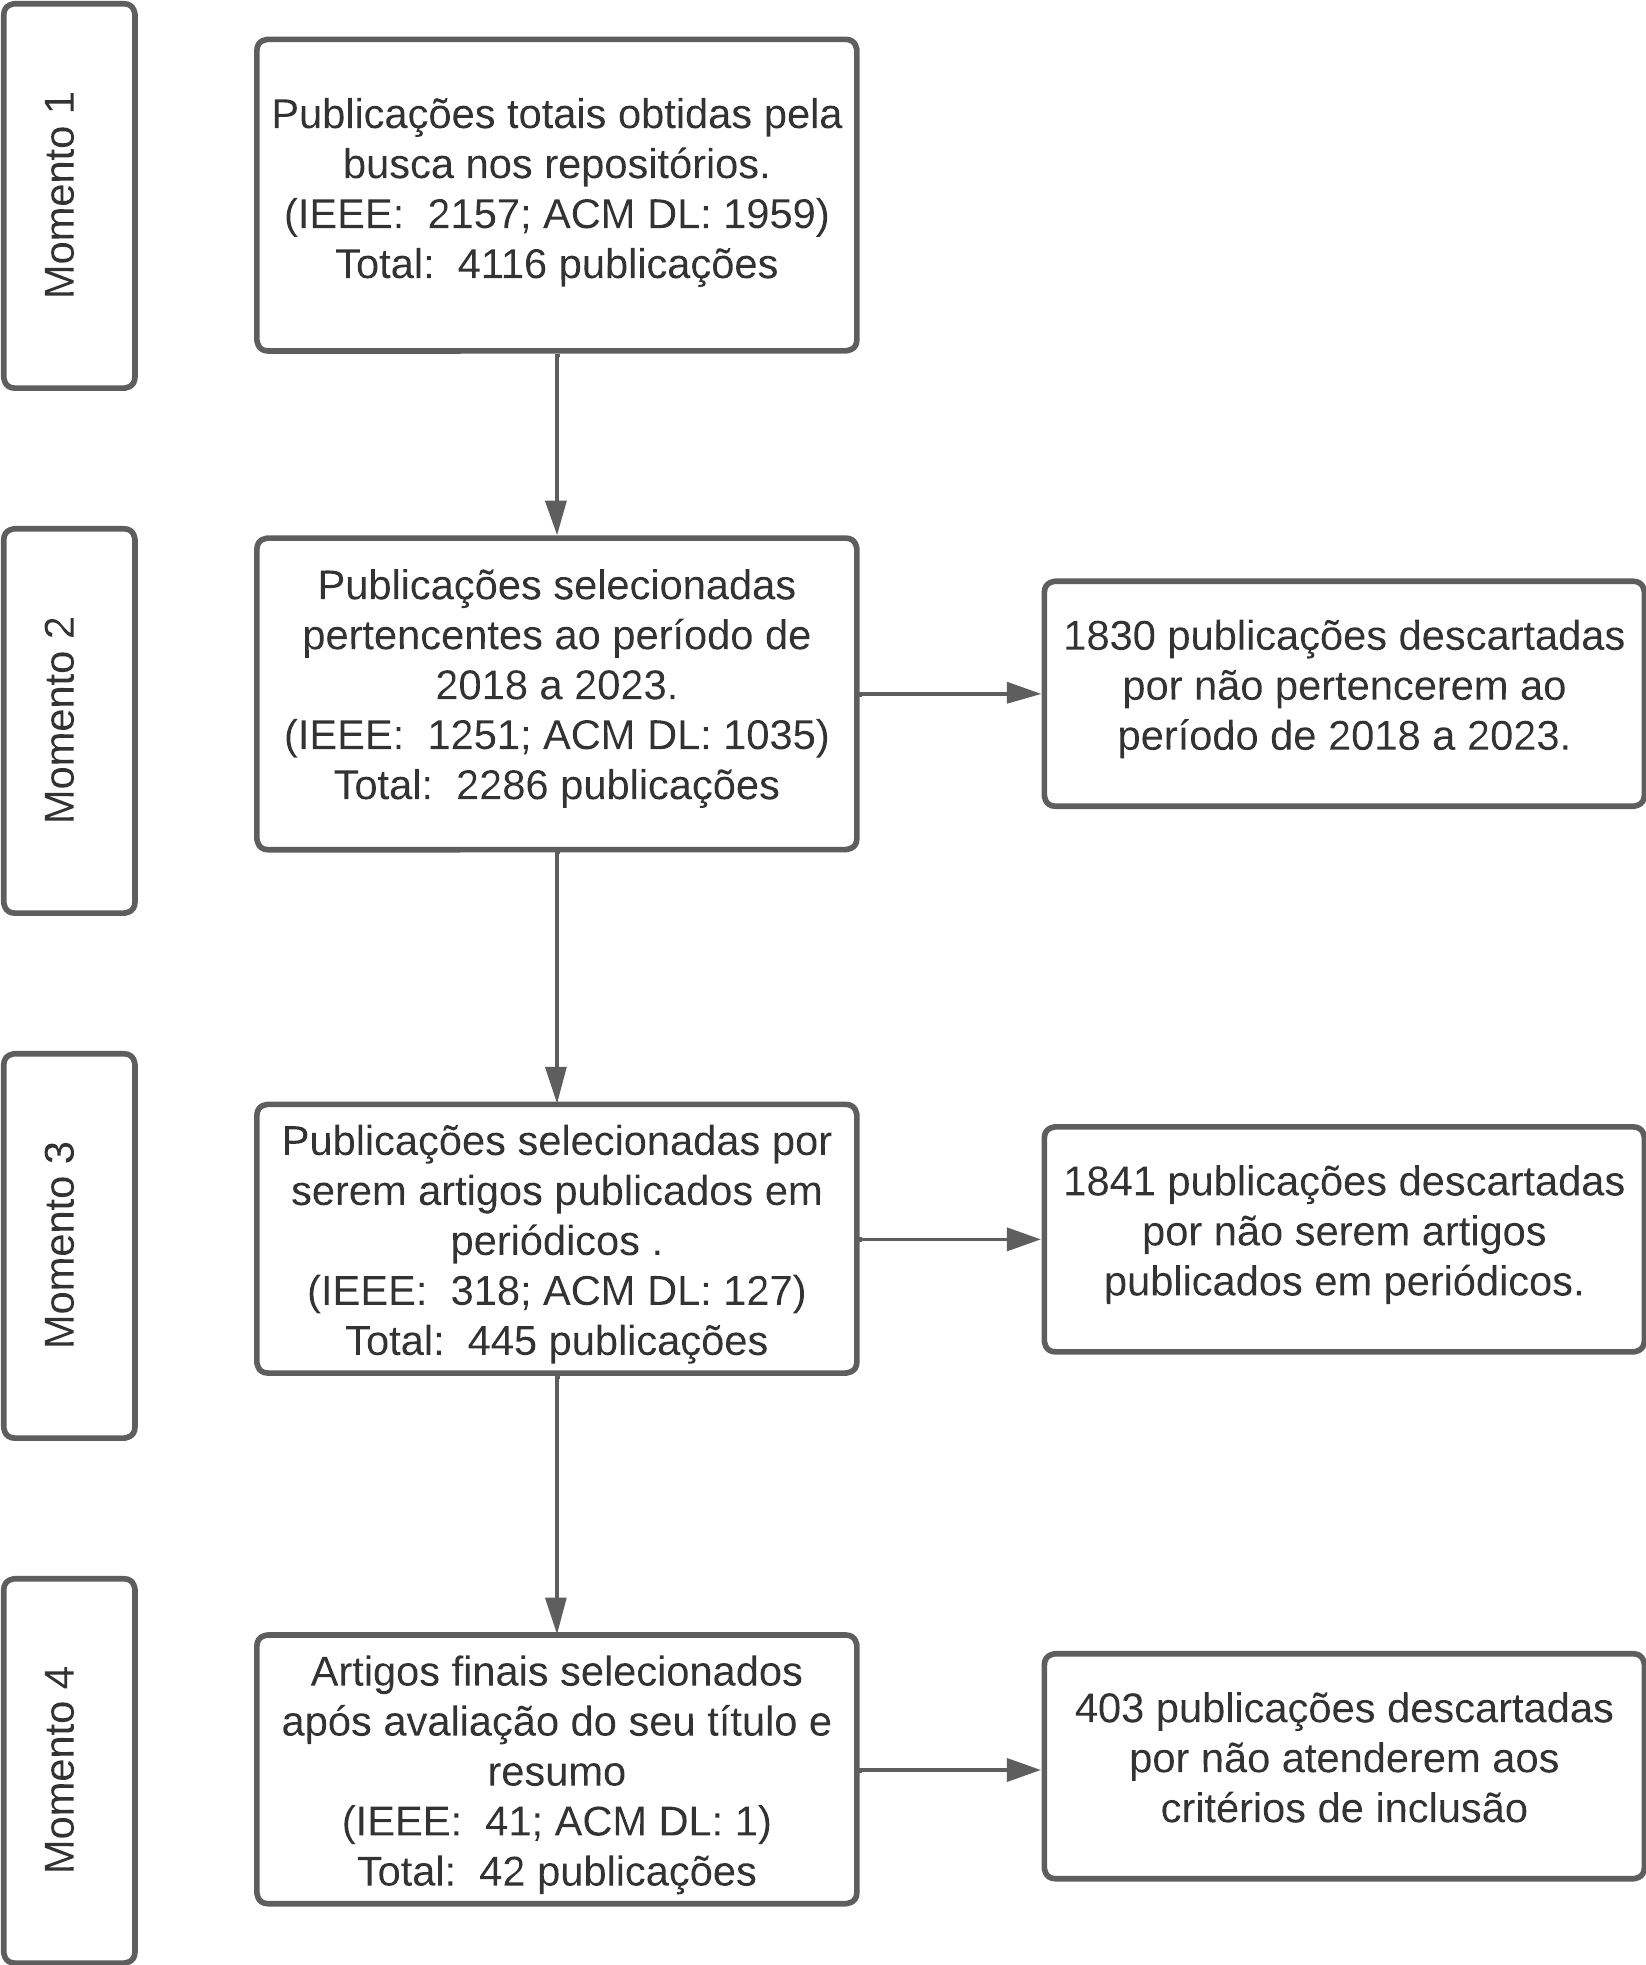
\includegraphics[scale=0.8]{diagramaResultadosLocalizacao.png}
    \caption*{Fonte: Autora (2023).}
    \label{fig:diagramaResultadosLocalizacao}
\end{figure}

Dentre as abordagens encontradas para localização de robôs autônomos móveis, 25 deles utilizavam a abordagem SLAM, pura ou com incrementos para melhorar o seu desempenho. No gráfico abaixo (Figura~\ref{fig:graficoPesquisaLocalizacao}) é possível observar todas as abordagens implementadas para a localização do robô em um ambiente interno, obtidas pela pesquisa realizada. Portanto, foi utilizado o algoritmo de localização e mapeamento simultâneo (SLAM) para auxiliar o robô a navegar de forma inteligente.

\begin{figure}[h]
    \centering
    \caption{Resultado da pesquisa bibliográfica de abordagens para localização de robôs autônomos móveis}
    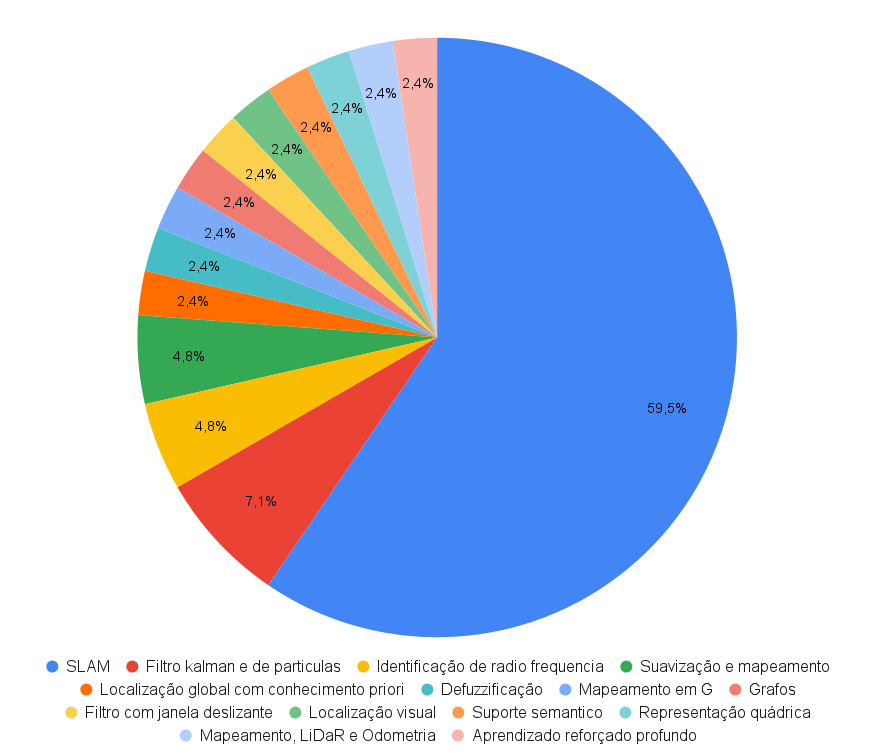
\includegraphics[scale=0.37]{resultadosAlgLocalizacao.png}
    \caption*{Fonte: Autora (2023).}
    \label{fig:graficoPesquisaLocalizacao}
\end{figure}

%%PERCEPÇÃO-----
De forma similar, a pesquisa bibliográfica que visava responder qual o instrumento mais utilizado para a percepção do ambiente pelo robô autônomo móvel, resultou em 1501 publicações totais, obtendo 33 artigos finais coerentes com os critérios de inclusão e exclusão definidos. Os resultados intermediários, conforme os momentos pré-estabelecidos, podem ser encontrado na Figura~\ref{fig:diagramaResultadosPercepcao}. 

\begin{figure}[h]
    \centering
    \caption{Resultado completo da pesquisa bibliográfica de instrumentos de percepção do ambiente}
    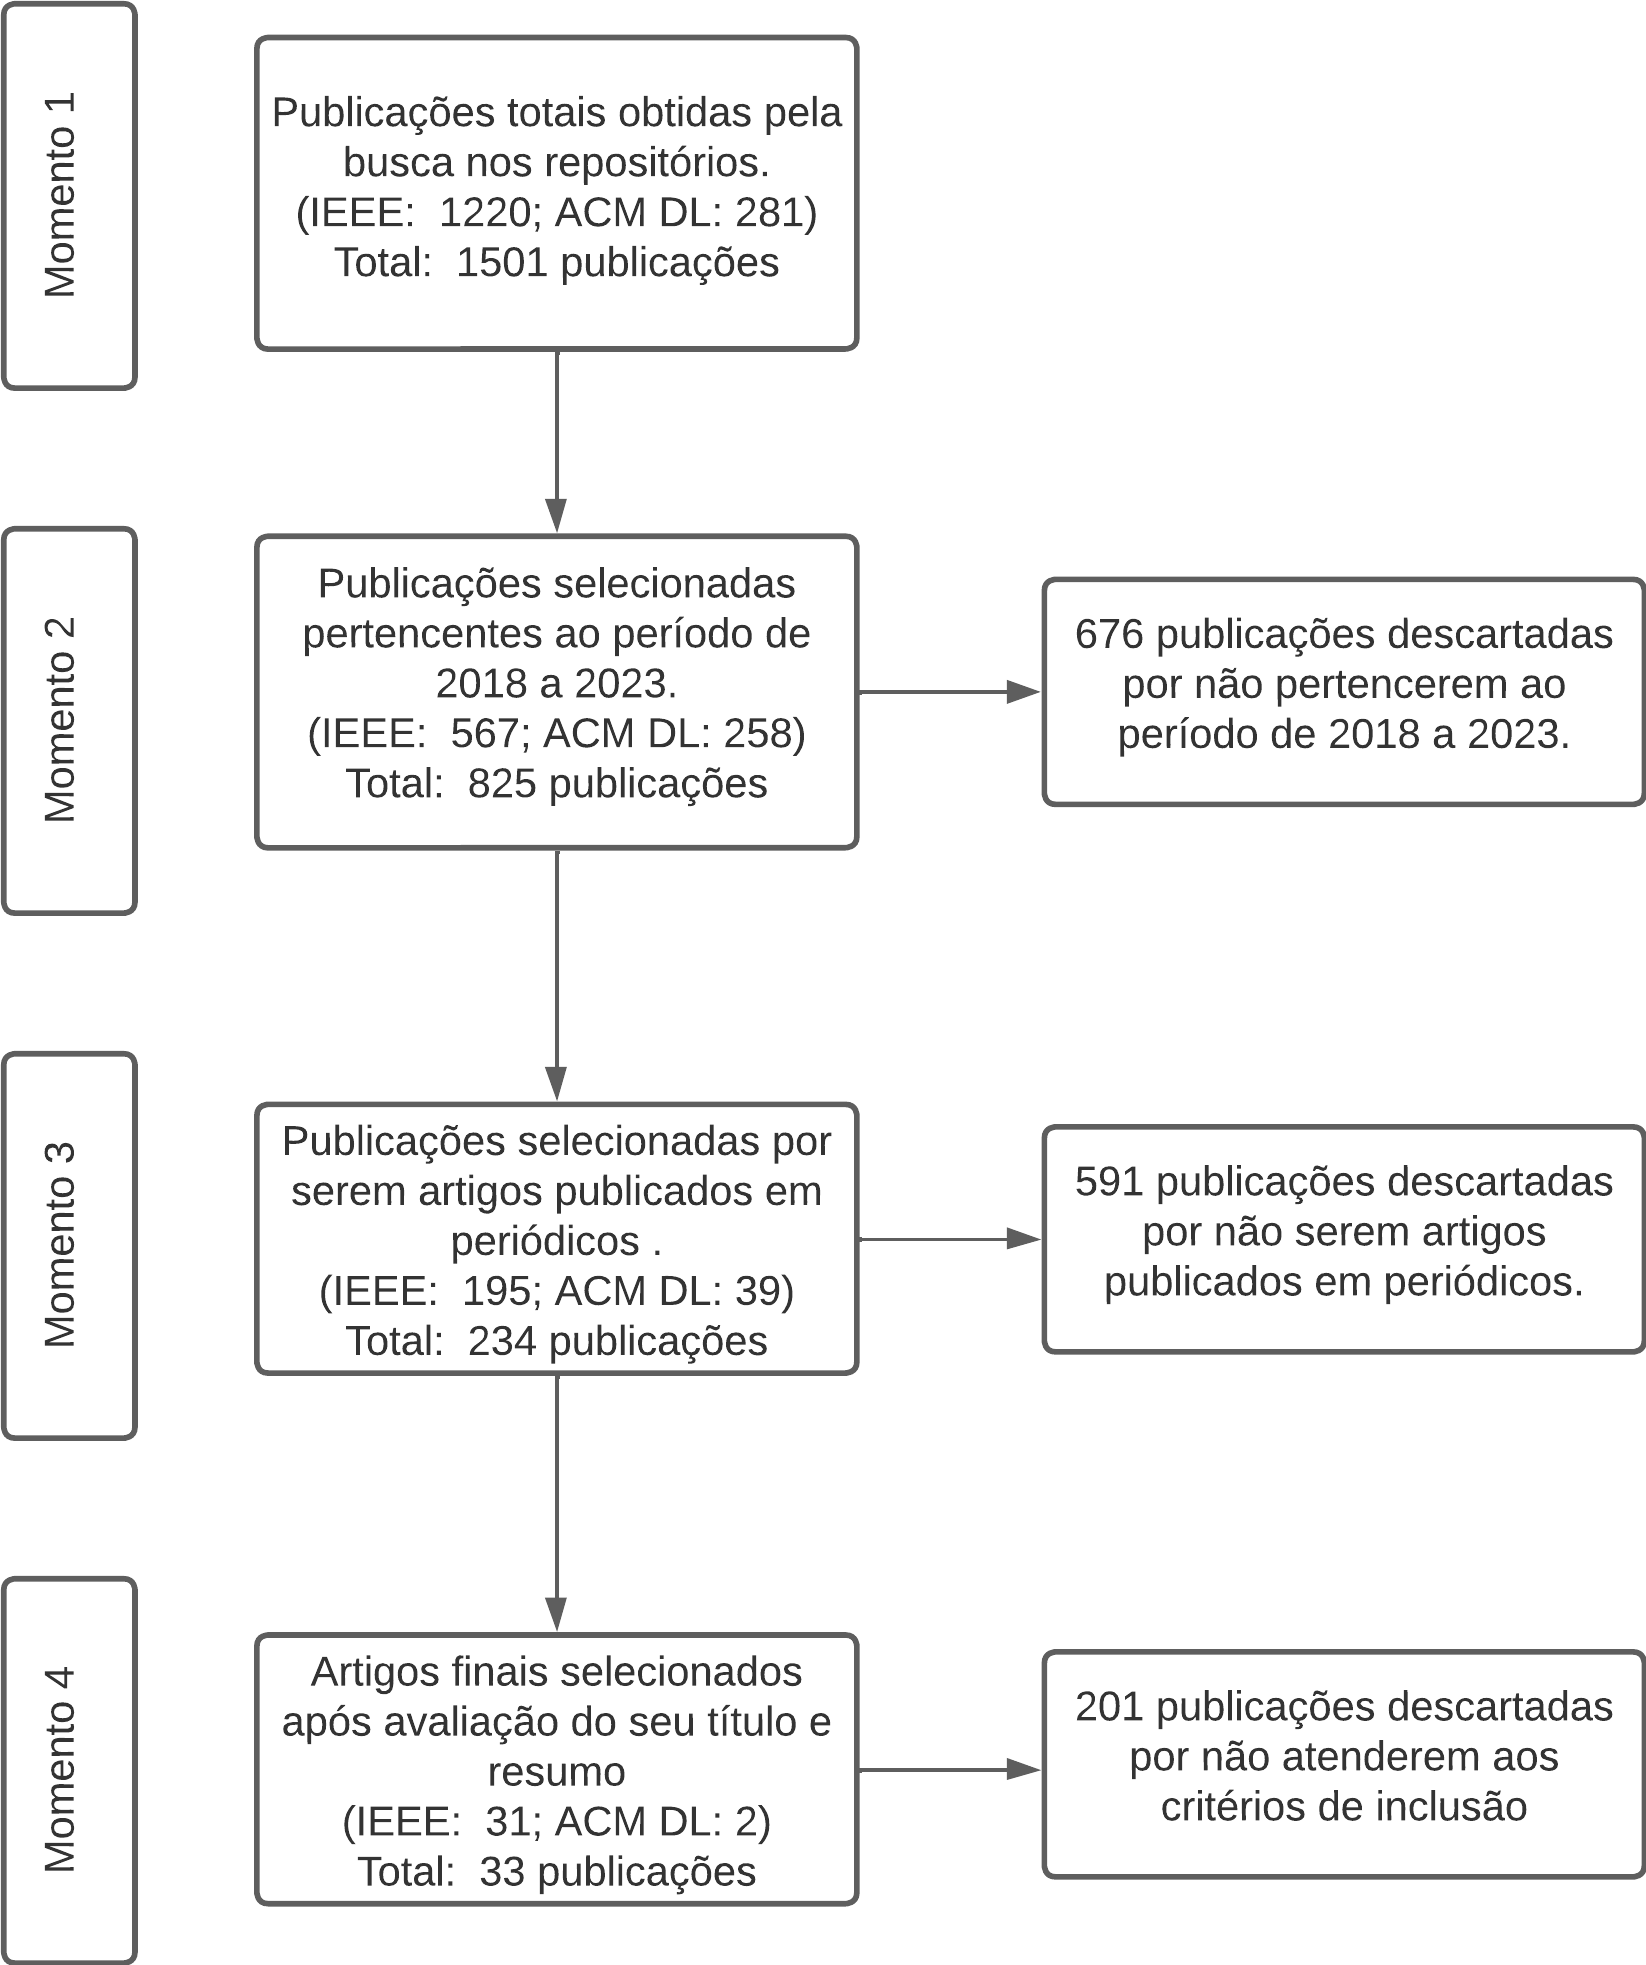
\includegraphics[scale=0.8]{diagramaResultadosPercepcao.png}
    \caption*{Fonte: Autora (2023).}
    \label{fig:diagramaResultadosPercepcao}
\end{figure}

Dentre as 33 publicações encontradas por essa pesquisa bibliográfica, 14 delas utilizam o sensor LiDaR e 5 utilizam a câmera, para o robô compreender o ambiente ao redor (Figura~\ref{fig:graficoPesquisaPercepcao}). Logo, foi optado a integração do sensor LiDaR para que o robô colete informações precisas do meio em que se encontra.

\begin{figure}[h]
    \centering
    \caption{Resultado da pesquisa bibliográfica de instrumentos de percepção do ambiente}
    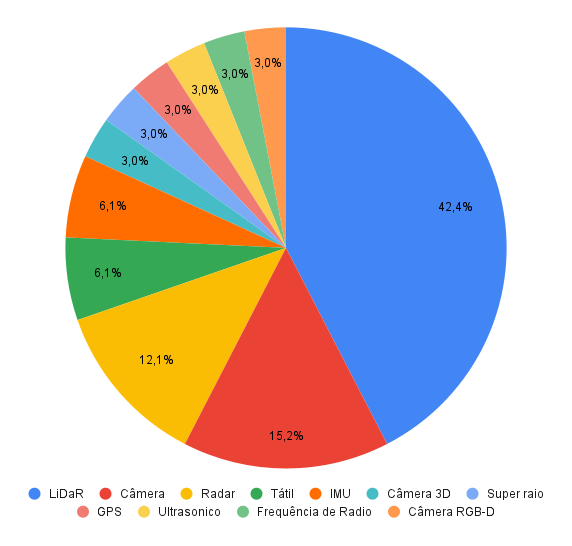
\includegraphics[scale=0.55]{resultadosPercepcao.png}
    \caption*{Fonte: Autora (2023).}
    \label{fig:graficoPesquisaPercepcao}
\end{figure}

%%LOCOMOÇÃO------- 
Como explicado anteriormente, a locomoção dos robôs autônomos móveis pode ser realizada com rodas ou pernas, similarmente a animais. Para o presente trabalho, foi optado utilizar rodas, ao apresentar uma melhor eficiência energética e não requerer técnicas para garantir equilíbrio do corpo do robô durante a movimentação, apresentando ser uma alternativa mais minimalista e intuitiva em sua concepção e implementação.  Com isso, o AtmosBot possui de 4 rodas de design padrão, dispostas a formar um quadrado na base do robô.

Como exposto no \chapterautorefname~\ref{cap-revisao-bibliografica}, o controle lógico do robô pode ser implementado com duas abordagens antagônicas: a inteligência artificial clássica sequencial e a arquitetura de subsunção com paralelismo. A fim de obter um robô com contato direto com as informações do ambiente em todos os seus módulos independentes, maior robustez, com capacidade de futuras incrementações, além de maior resiliência e menor tempo de resposta a mudanças no ambiente, foi optado o uso da arquitetura de subsunção, com um grau de liberdade para possíveis adaptações necessárias caso demonstre ser mais adequado para a proposta.

Por fim, o ambiente também deve ser definido para que o modelo do robô seja correto. Esse robô deve atuar em um ambiente interno e dinâmico, semelhante a um domicílio acessível. Ou seja, o robô consegue atuar apenas em ambientes com uma iluminação controlada, com obstáculos  (parede, portas fechadas, móveis e outros objetos), com  mudanças na disposição dos artefatos presentes, além de não possuir degraus com altura acima de 1 centímetro.

\section{Especificação de Requisitos}

Os requisitos de um sistema são características que esse sistema necessita para o seu funcionamento. Os requisitos básicos devem ser identificados previamente ao desenvolvimento, no intuito de compreender ao máximo os limites do sistema e as funcionalidades que devem ser alcançadas \cite{pressman}.

Dito isso, foi  levantada uma série de requisitos do sistema completo, incluindo a simulação do ambiente e do robô proposto. Esse conjunto de requisitos levantados detalham as possíveis ações do robô e suas características mais intrínsecas, além de conformidades do ambiente. 

Em específico, foram levantados requisitos funcionais e não funcionais para o robô autônomo móvel proposto. Essas especificações abordam a movimentação do robô ao longo da sua trajetória no ambiente, como sua capacidade de evitar os obstáculos e conter uma velocidade segura para os humanos e a propriedade presente no meio inserido.

Ademais, foram levantados requisitos não funcionais para o ambiente, explicitando as necessidades do local de atuação do robô proposto. Dentre elas, foram destacadas a verossimilhança com domicílios comuns e sua dinamicidade como um meio convivido por seres.

A fim de expor todos os requisitos, foi elaborado um documento de Especificação de Requisitos do Sistema  com base nas práticas recomendadas pela norma IEEE Std 830-1998, Práticas Recomendadas para Especificações de Requisitos de Software da IEEE,  que pode ser encontrado na íntegra no \appendixautorefname~\ref{appendix-requisitos}.

\section{Modelagem do Sistema}

O AtmosBot como navegador autônomo cumpre seu objetivo de navegação eficiente a partir de duas grandes etapas: espera no ponto de partida e exploração do ambiente

A exploração do ambiente pode ser subdividida em quatro tarefas importantes executadas paralelamente: 1) a locomoção pelo espaço, 2) a coleta de informações do meio para se localizar, 3) o mapeamento do ambiente, 4) o desvio dos obstáculos fixos e dinâmicos. Todas essas funcionalidades podem ser caracterizadas por estados conforme demonstrados na Figura~\ref{fig:estados}. 

\begin{figure}[h]
    \centering
    \caption{Estados principais do AtmosBot}
    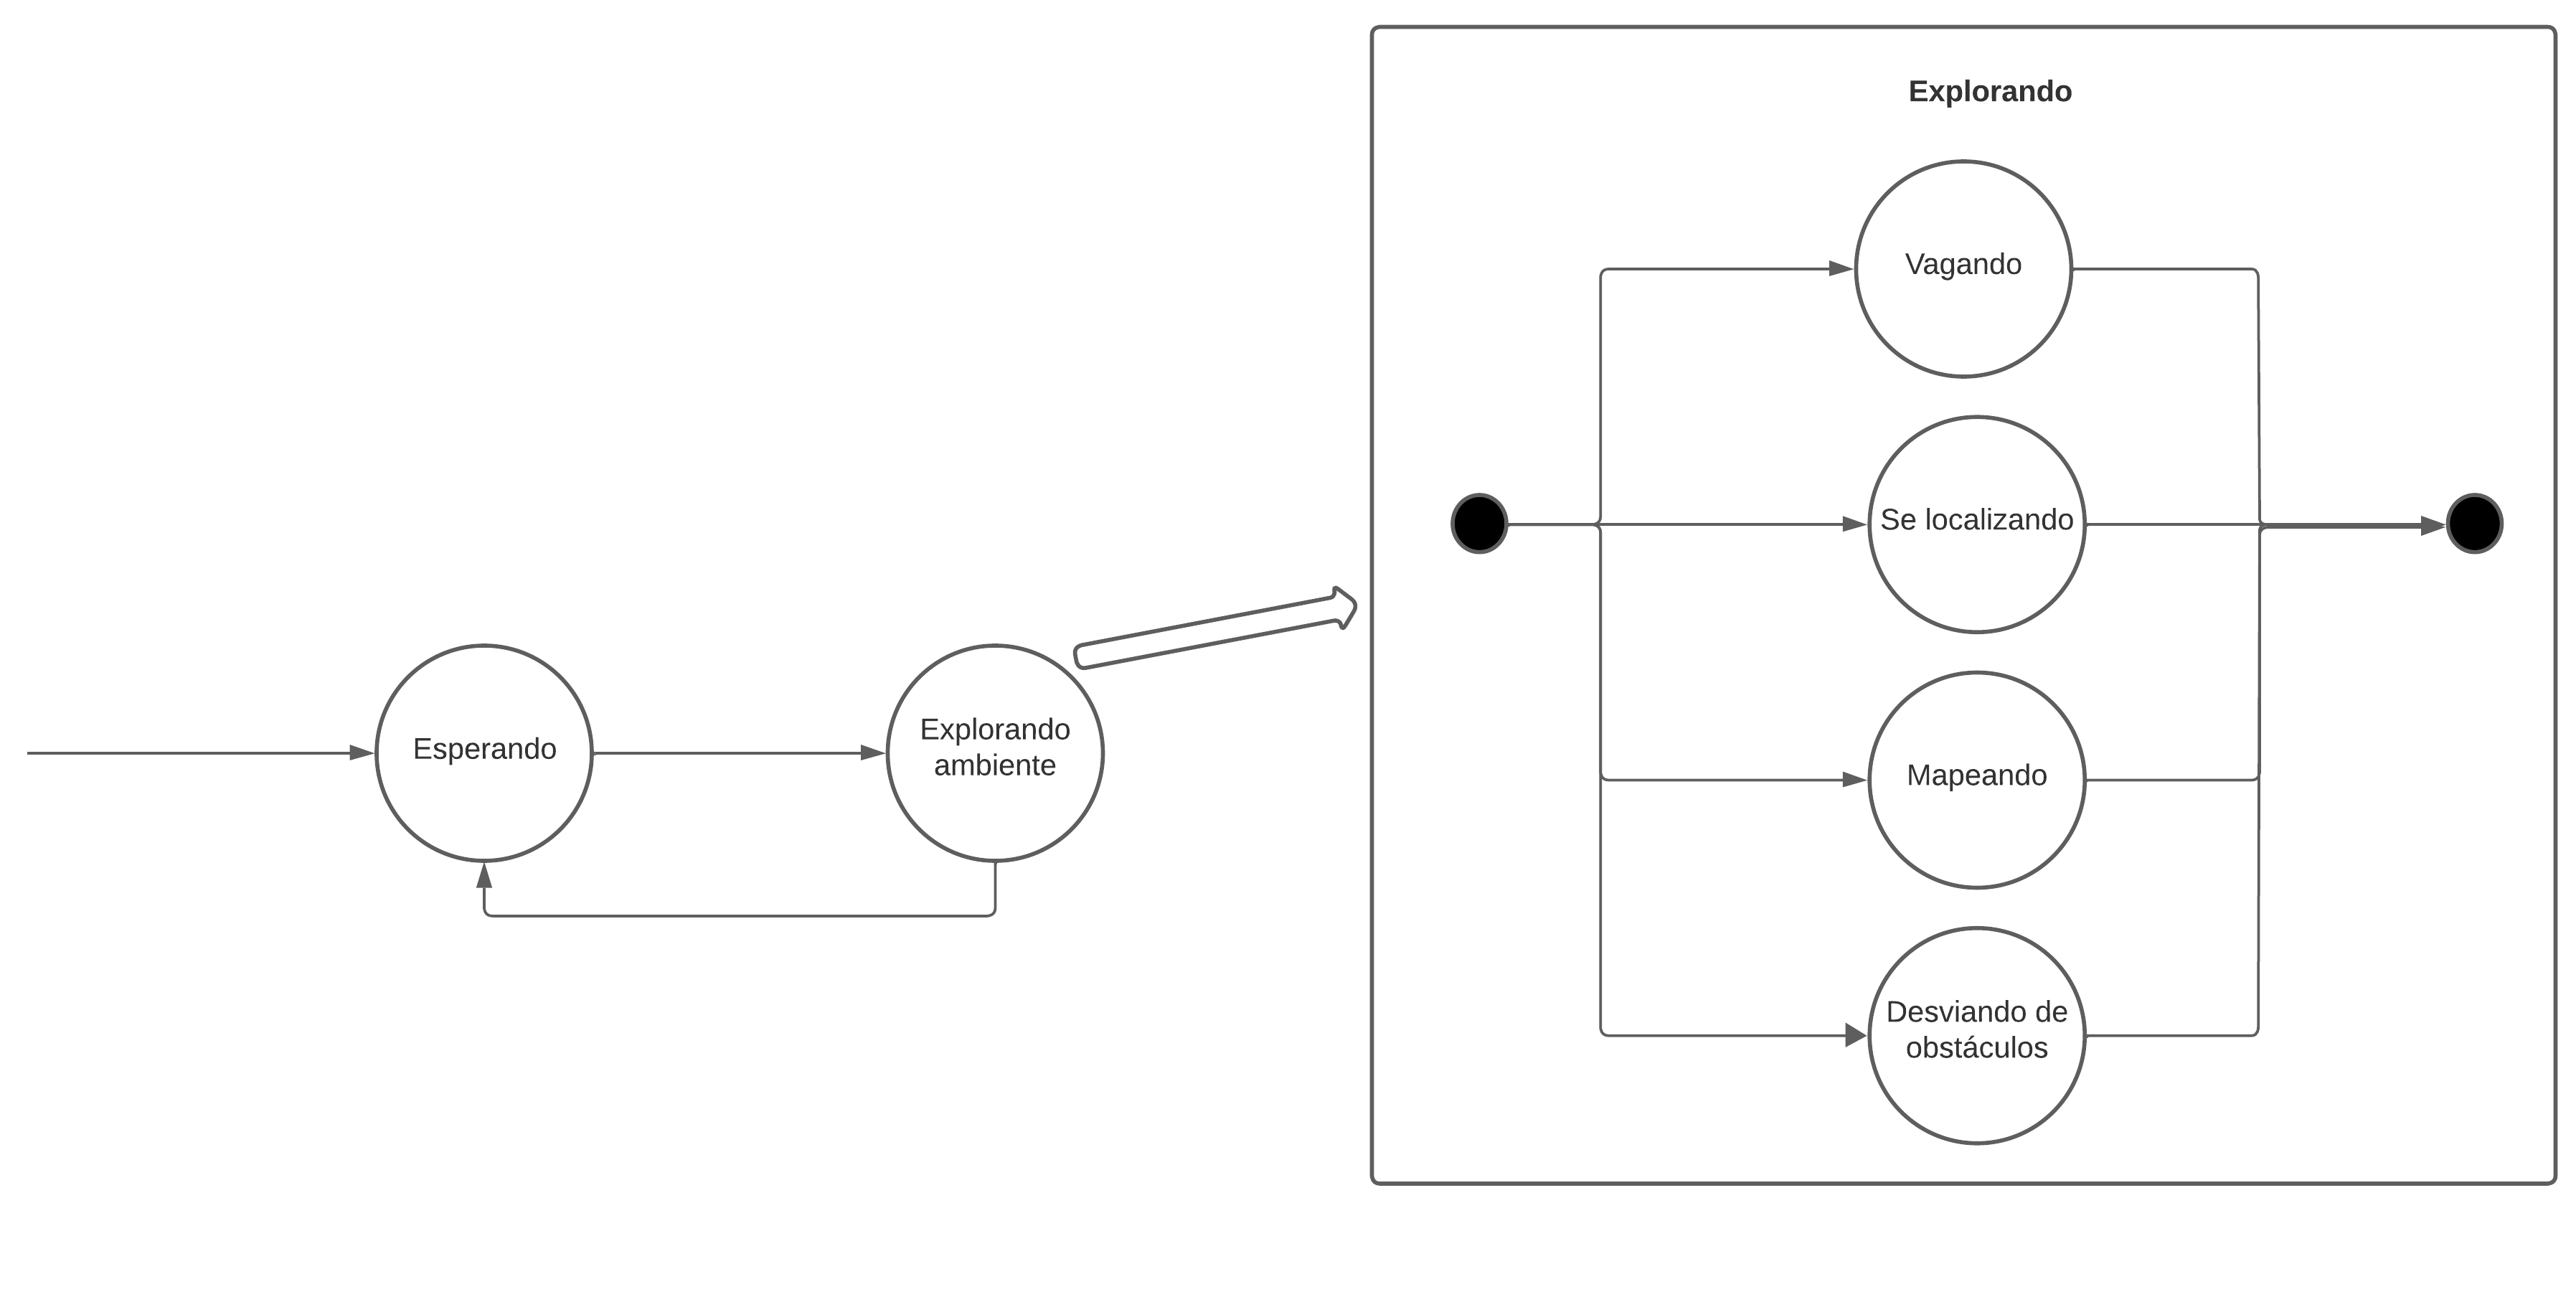
\includegraphics[scale=0.45]{estados.png}
    \caption*{Fonte: Autora (2023).}
    \label{fig:estados}
\end{figure}


Inicialmente, o sistema deve estar em modo de espera para começar sua tarefa. Passado o tempo padrão de espera para que todos os seus processamentos estejam preparados, o robô inicia sua tarefa de explorar o ambiente, vagando pelo meio sem colidir com os obstáculos e coletando informações sobre a sua posição. 

Este modelo permite a adição de outras funcionalidades em paralelo com o módulo de navegação, conforme a aplicação da abordagem de subsunção, que torna as unidades independentes. Apesar de serem unidades independentes, o módulo de navegação autônoma e outros possíveis módulos devem ser interligados com transmissão de informações cruciais entre si, além de se comunicarem com o próprio ambiente onde o robô se encontra. Essa interação entre os subsistemas, o sistema geral e o ambiente, pode ser analisada visualmente através da Figura~\ref{fig:blocos}.  

Em paralelo com a execução de outras possíveis funcionalidades que poderão ser incrementadas, o módulo de navegação recebe as informações que os instrumentos de percepção coletam do ambiente e as suas sub-camadas utilizam esse conhecimento para definir a atividade dos atuadores (os motores e consequentemente as rodas). Uma vez que o robô atua no ambiente, as informações dele mudam, pois o robô se encontra em outra posição, tornando um ciclo fechado entre atuação e percepção do meio.

\begin{figure}[h]
    \centering
    \caption{Diagrama de blocos do modelo}
    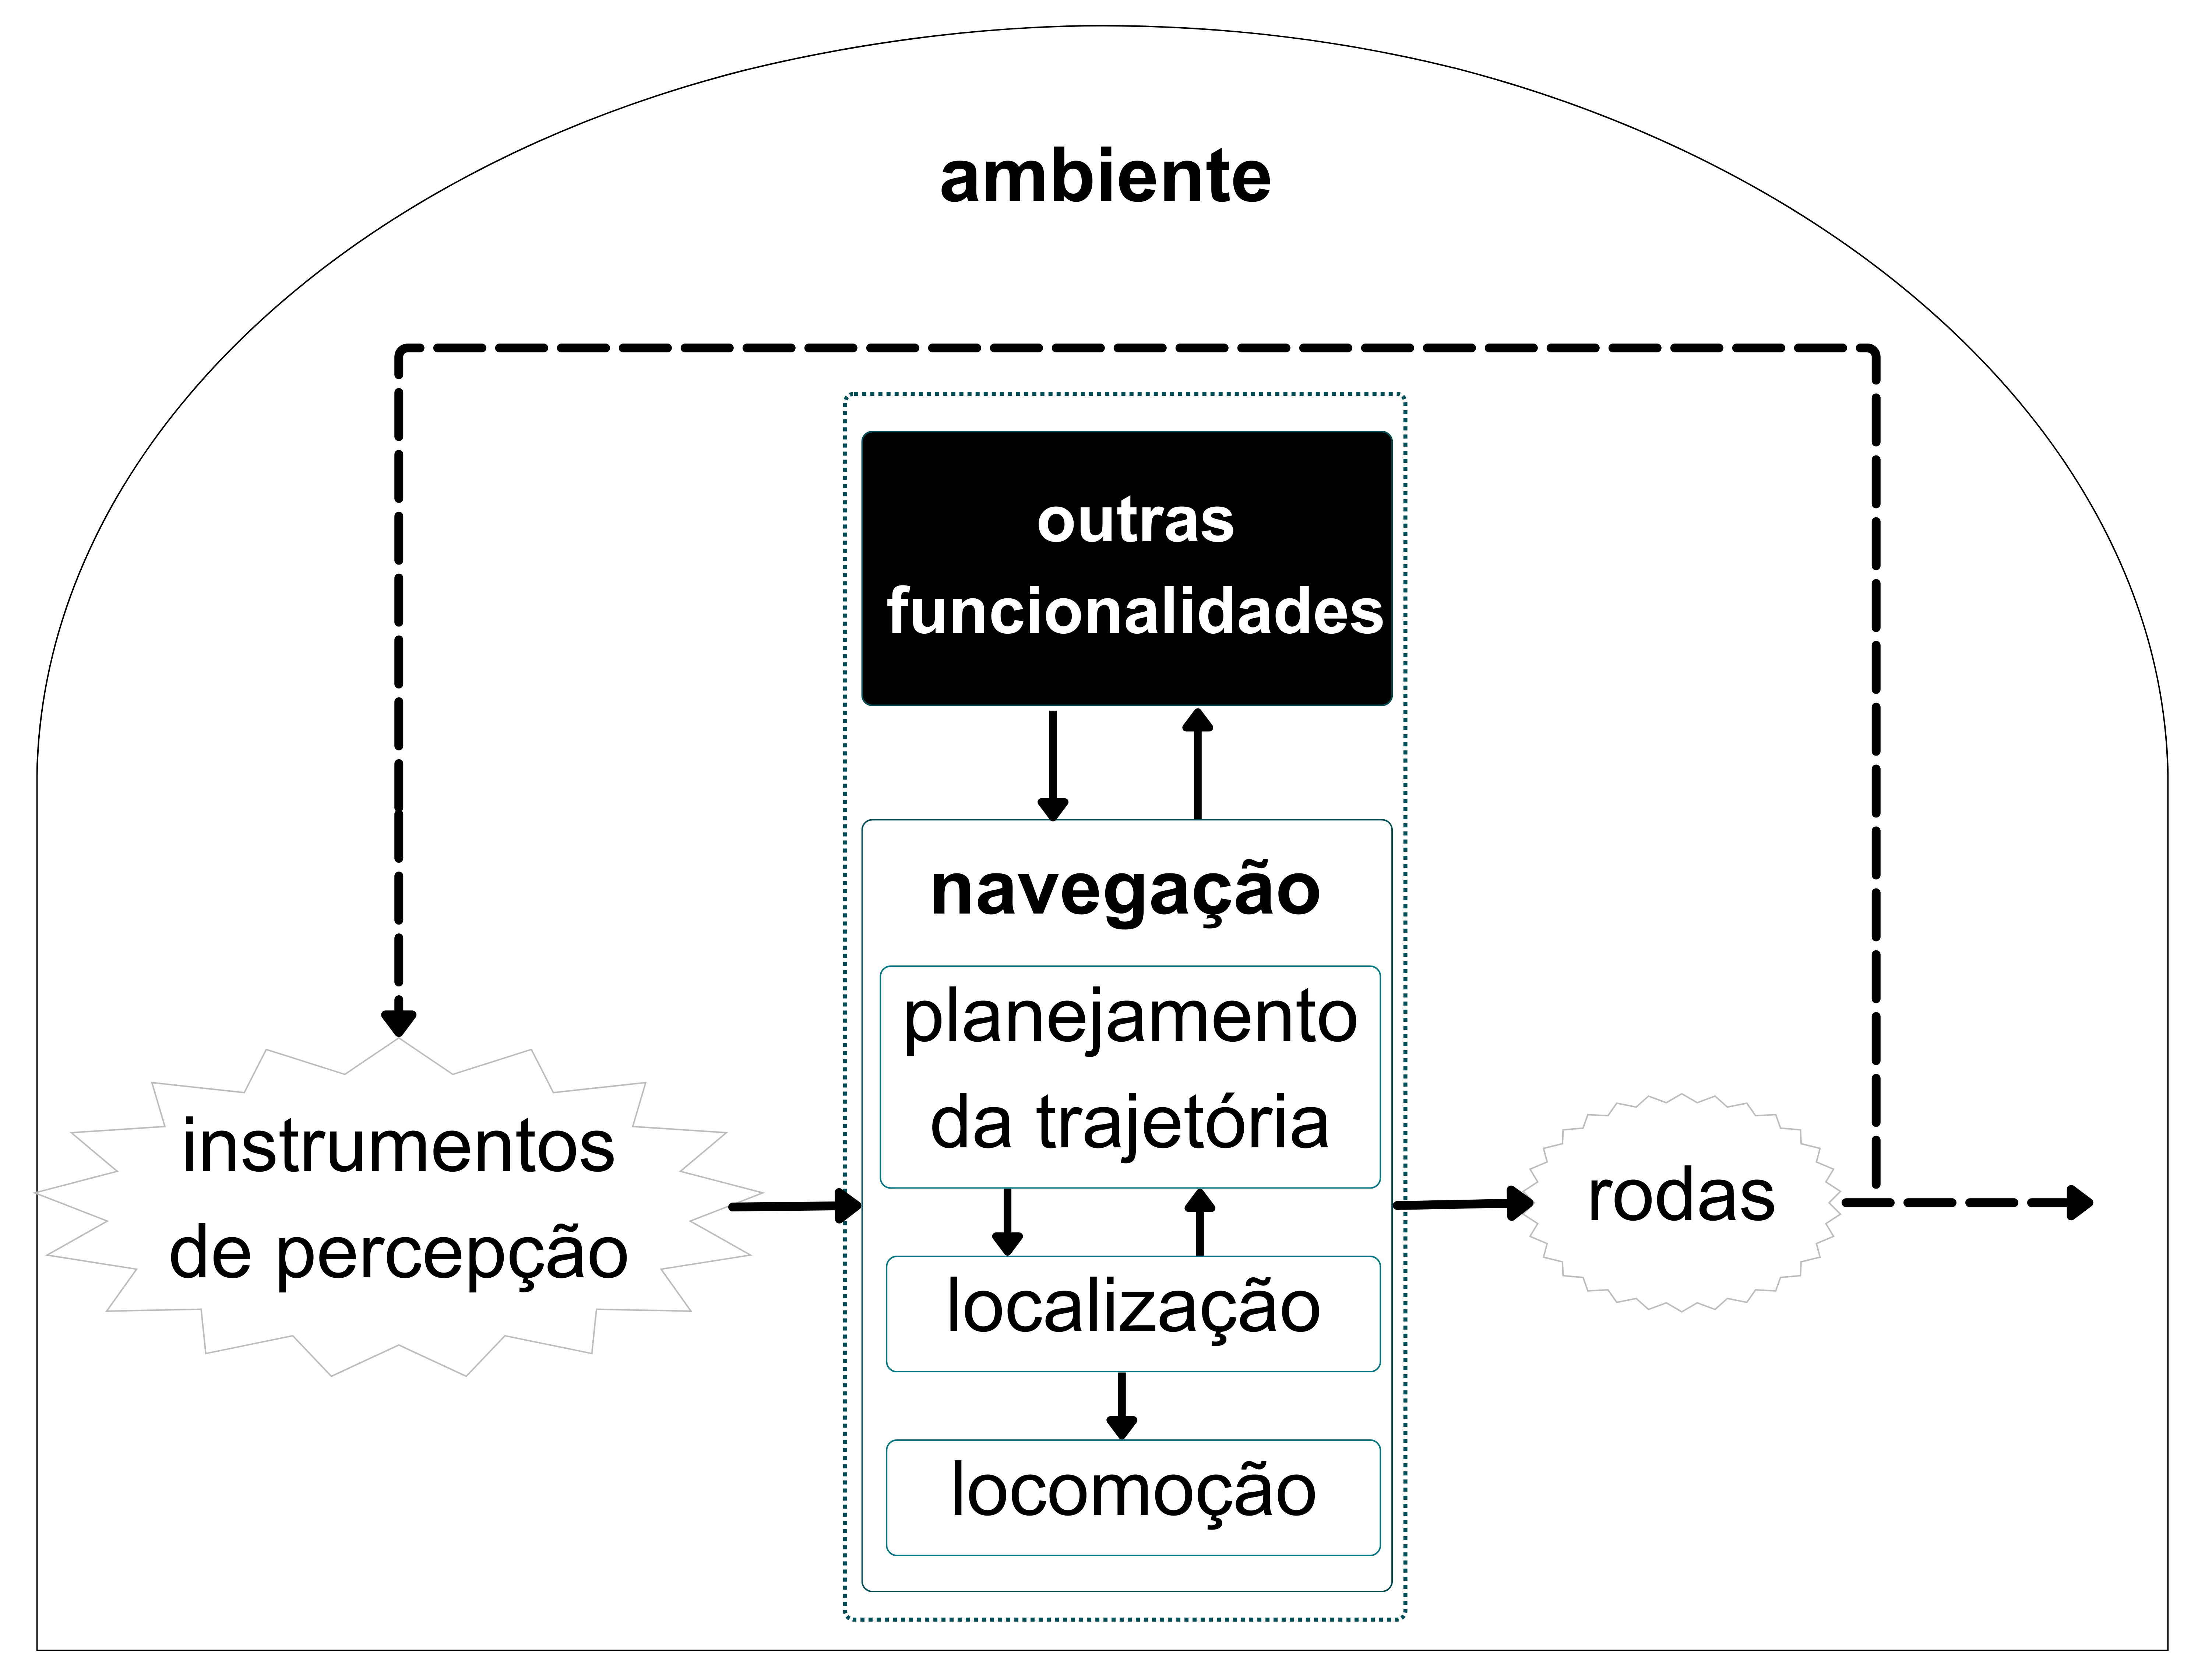
\includegraphics[scale=0.08]{blocos.png}
   
    \caption*{Fonte: Autora (2023).}
    \label{fig:blocos}
\end{figure}


\section{Implementação da Proposta}
A implementação da proposta pode ser separada em três elementos: i) a simulação; ii) o controle do robô; iii) integração de todos os componentes. O desenvolvimento de cada elemento é explicado detalhadamente a seguir.

\subsection{Simulação}
A simulação é responsável por permitir a recriação da realidade de forma mais verossímil possível. Para isso, cada aspecto dos elementos reais deve ser descrito com alta riqueza de detalhes, para serem representados na simulação com maior semelhança. Para o simulador Gazebo, essa descrição é realizada mediante arquivos SDF (do inglês Formato de Descrição de Simulação) que compõe todas as características necessárias para a definição de elementos do ambiente e do robô. Entre essas características, são descritas o comportamento dos componentes perante as leis da física, além de tamanho, cor, articulações e movimento.

Visto que uma das maiores vantagens do simulador Gazebo é a sua comunidade ativa de desenvolvedores usários que continuamente disponibiliza novos modelos de robôs e ambientes, foi possível criar o robô AtmosBot baseado no modelo disponibilizado por \citet{modeloRobo}. A fim de obter uma melhor resolução na simulação, em conjunto com os arquivos SDF, cada parte do robô (rodas, base e estrutura vertical) foi renderizada por dados de malha tridimensional (MESH) elaborados e modificados no programa de design 3D Blender.

Assim como o uso de um modelo de robô disponibilizado pela comunidade do Gazebo, foi possível montar o domicílio simulado com modelos publicados pela plataforma "AWS Robot Maker" da Amazon, destinada a executar e automatizar simulações sem necessitar lidar com a infraestrutura \cite{aws, modeloAmbiente}.

A simulação se torna completa ao combinar o ambiente montado com o robô elaborado. Para compreender a visão do robô ao longo da simulação, foi utilizado o programa RVIZ que permite visualizar os processos ocorrendo com o robô, como a sua odometria, velocidade e capturas de sensores.

\subsection{Navegação Autônoma}

A navegação autônoma do AtmosBot foi subdividida em duas principais partes: i) vagar pelo ambiente sem colisões e ii) mapeamento e localização durante exploração do ambiente.

A fim de fazer o robô se locomover pelo ambiente simulado de forma livre sem colidir com os móveis e paredes ao longo do caminho, foi desenvolvido um algoritmo, na linguagem C++, capaz de compreender obstáculos à sua frente. Para isso, são capturadas as leituras do sensor LiDaR, posicionado na dianteira do robô, com intuito de validar se existe um obstáculo à sua frente e os possíveis cenários para rotação do robô (Figura~\ref{fig:fluxogramaEvitarObstaculos}).  Uma vez que foi identificado uma nova rota, são definidas as velocidades linear (para seguir em frente ou dar ré) e angular (para rotacionar), conforme necessário.

\begin{figure}[h]
    \centering
    \caption{Fluxograma do algoritmo de vagar sem colidir}
    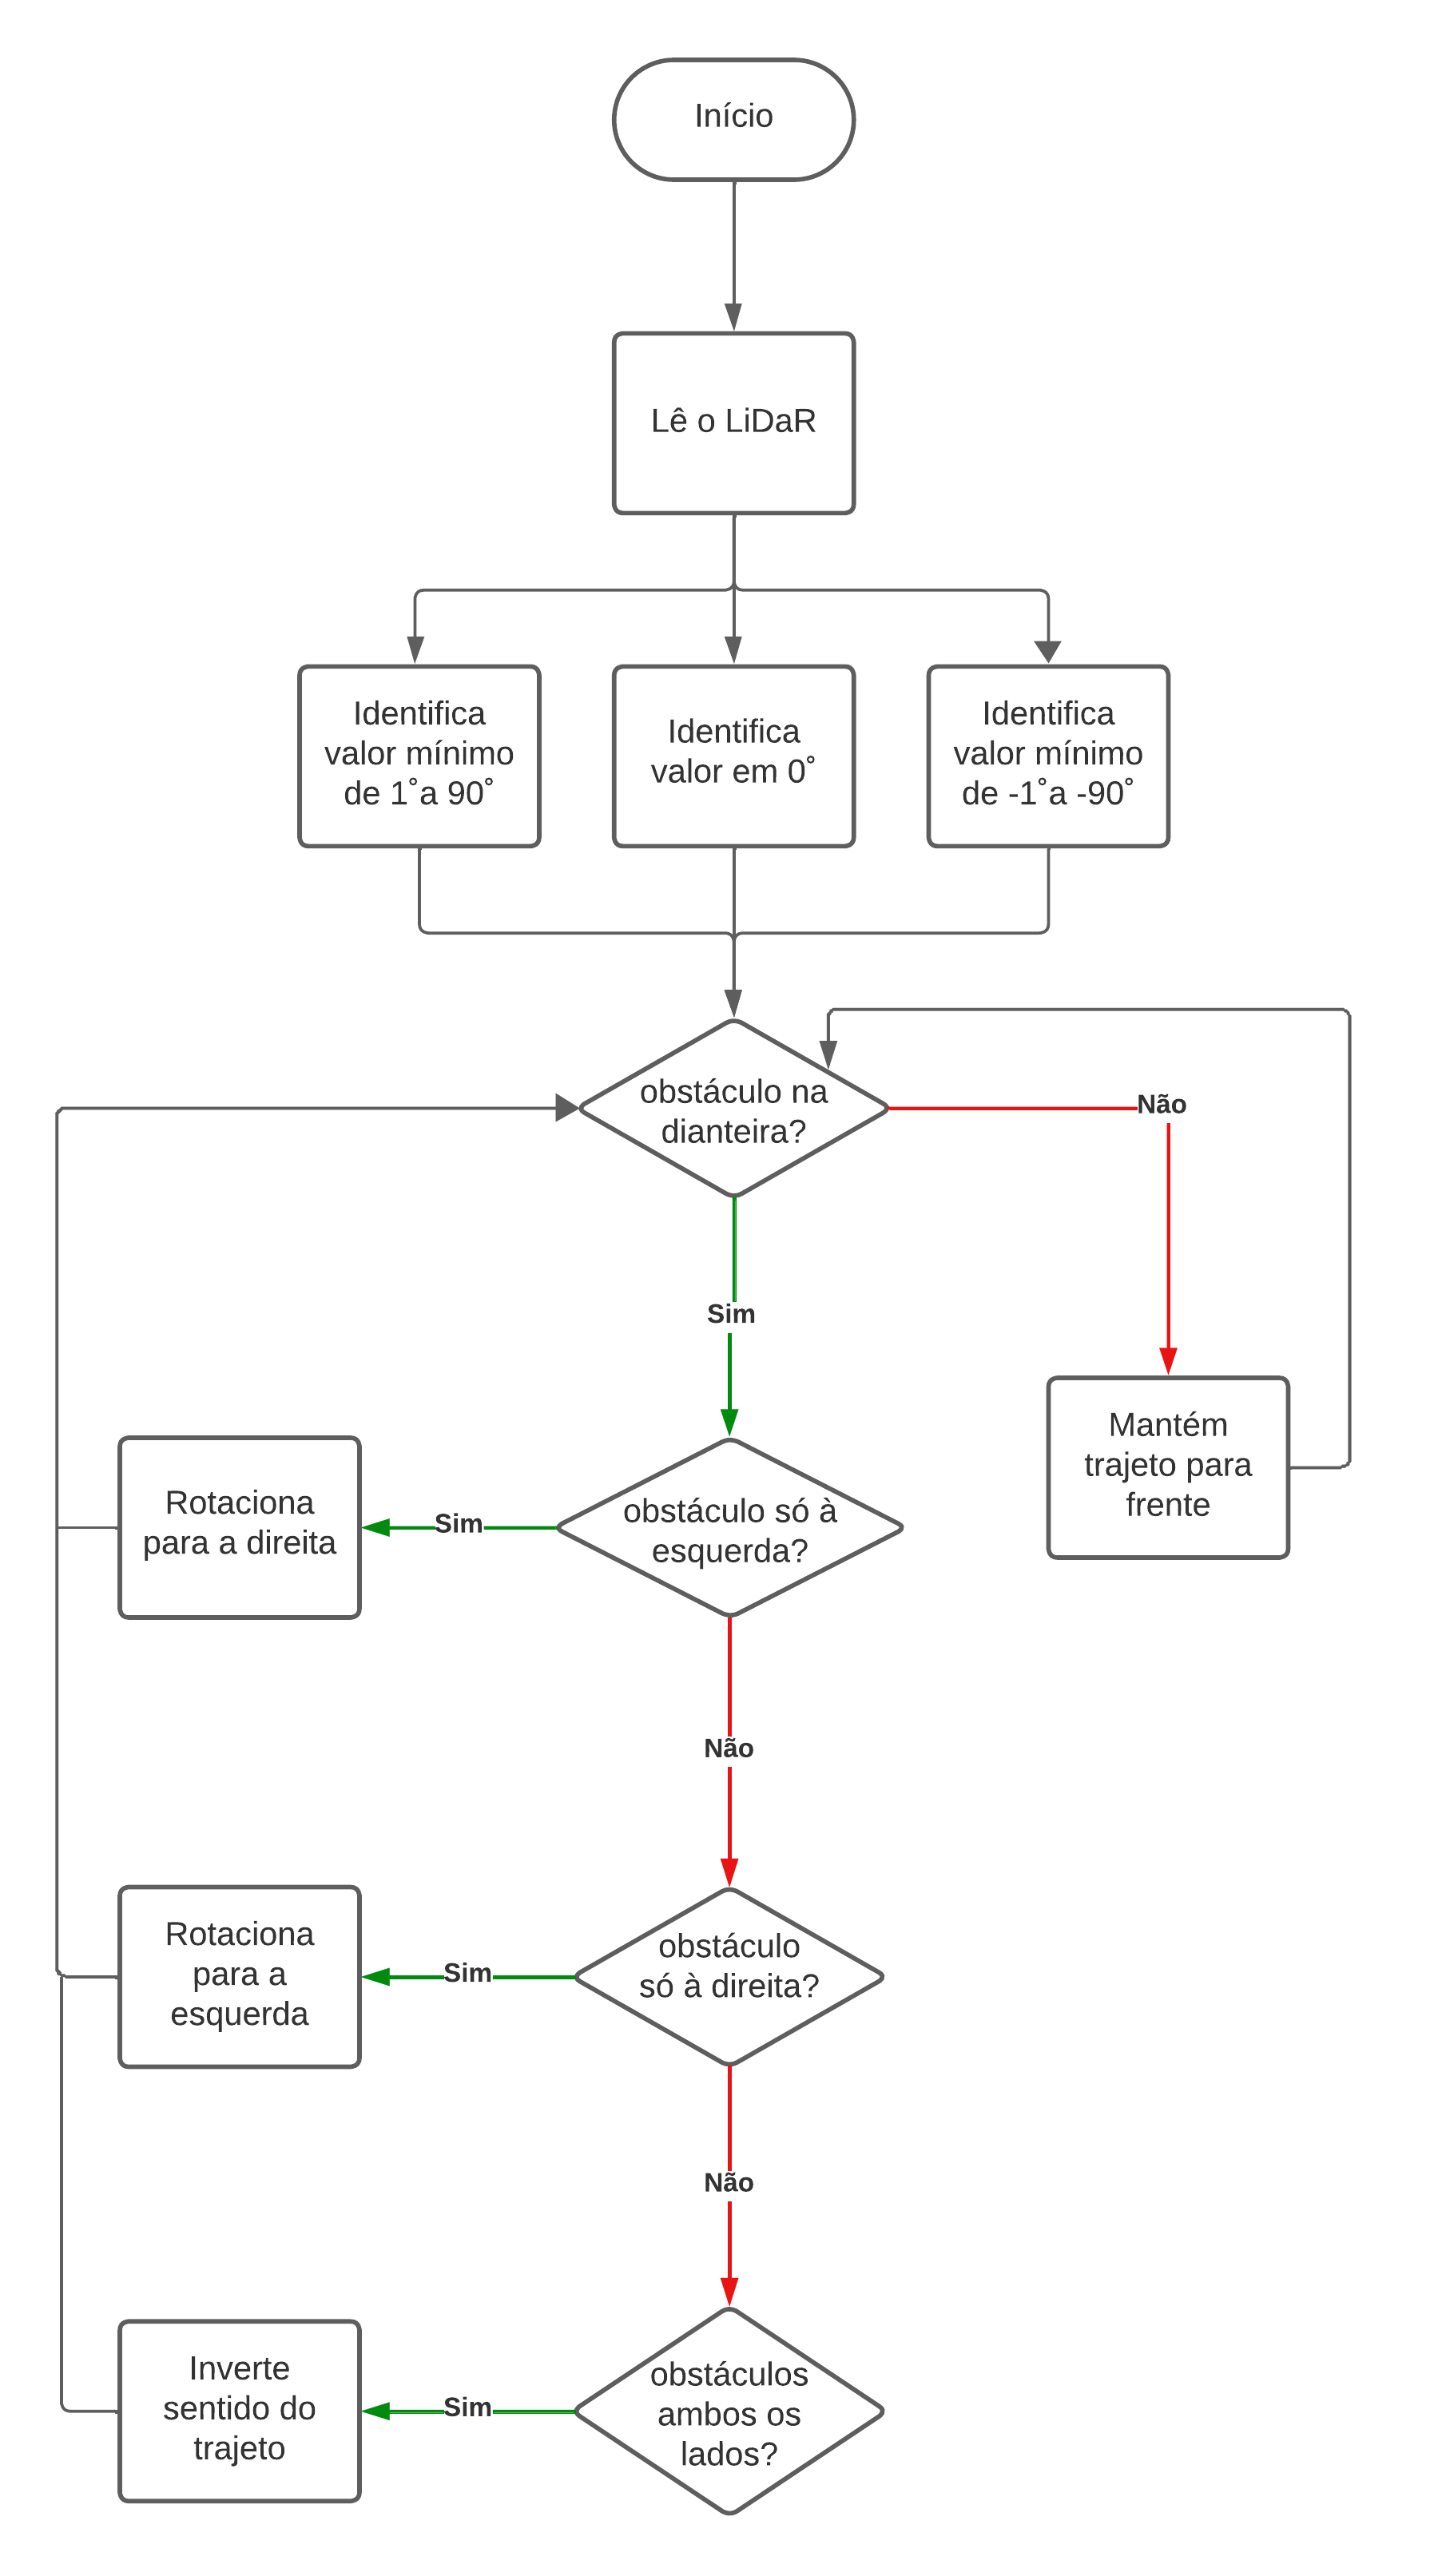
\includegraphics[scale=0.5]{fluxogramaEvitarObstaculos.png}
    
    \caption*{Fonte: Autora (2023).}
    \label{fig:fluxogramaEvitarObstaculos}
\end{figure}

Para o mapeamento do ambiente e a localização do robô, foi possível usufruir de uma das maiores vantagens do Sistema Operacional de Robô (ROS): as variadas bibliotecas disponíveis que executam diversas funcionalidades. As bibliotecas utilizadas para realizar o comportamento compatível com a abordagem SLAM, foram a  Slam Toolbox  e Nav2 \cite{nav2, slamtoolbox}.

A biblioteca Slam Toolbox foi criada no intuito de disponibilizar um conjunto de ferramentas para aplicar o SLAM em duas dimensões \cite{slamtoolbox}. Para o referente trabalho, a biblioteca é executada com o perfil de mapeamento em modo assíncrono, utilizando as informações do sensor LiDaR e odometria.  O modo assíncrono permite que o mapa a ser criado e atualizado utilize apenas informações confiáveis dos sensores, tornando a navegação mais robusta. A partir dessa execução, é obtido o mapa do ambiente e o posicionando do robô neste mapa conforme as novas leituras dos sensores.

O mapa disponibilizado pela execução biblioteca Slam Tollbox é acessado pela biblioteca Nav2. Essa por sua vez, é uma coleção de utensílios facilitadores para a navegação autônoma de um robô \cite{nav2}. Com o mapa criado pela biblioteca Slam Toolbox, o Nav2 consegue reconhecer a posição do robô. A partir disso, é possível definir um ponto de destino, permitindo que o Nav2  envie comando de velocidade  para o robô, a fim de conduzi-lo até o destino selecionado (Figura~\ref{fig:fluxogramaComando}).

\begin{figure}[h]
    \centering
    \caption{Fluxograma da interação entre Slam Toolbox e Nav2}
    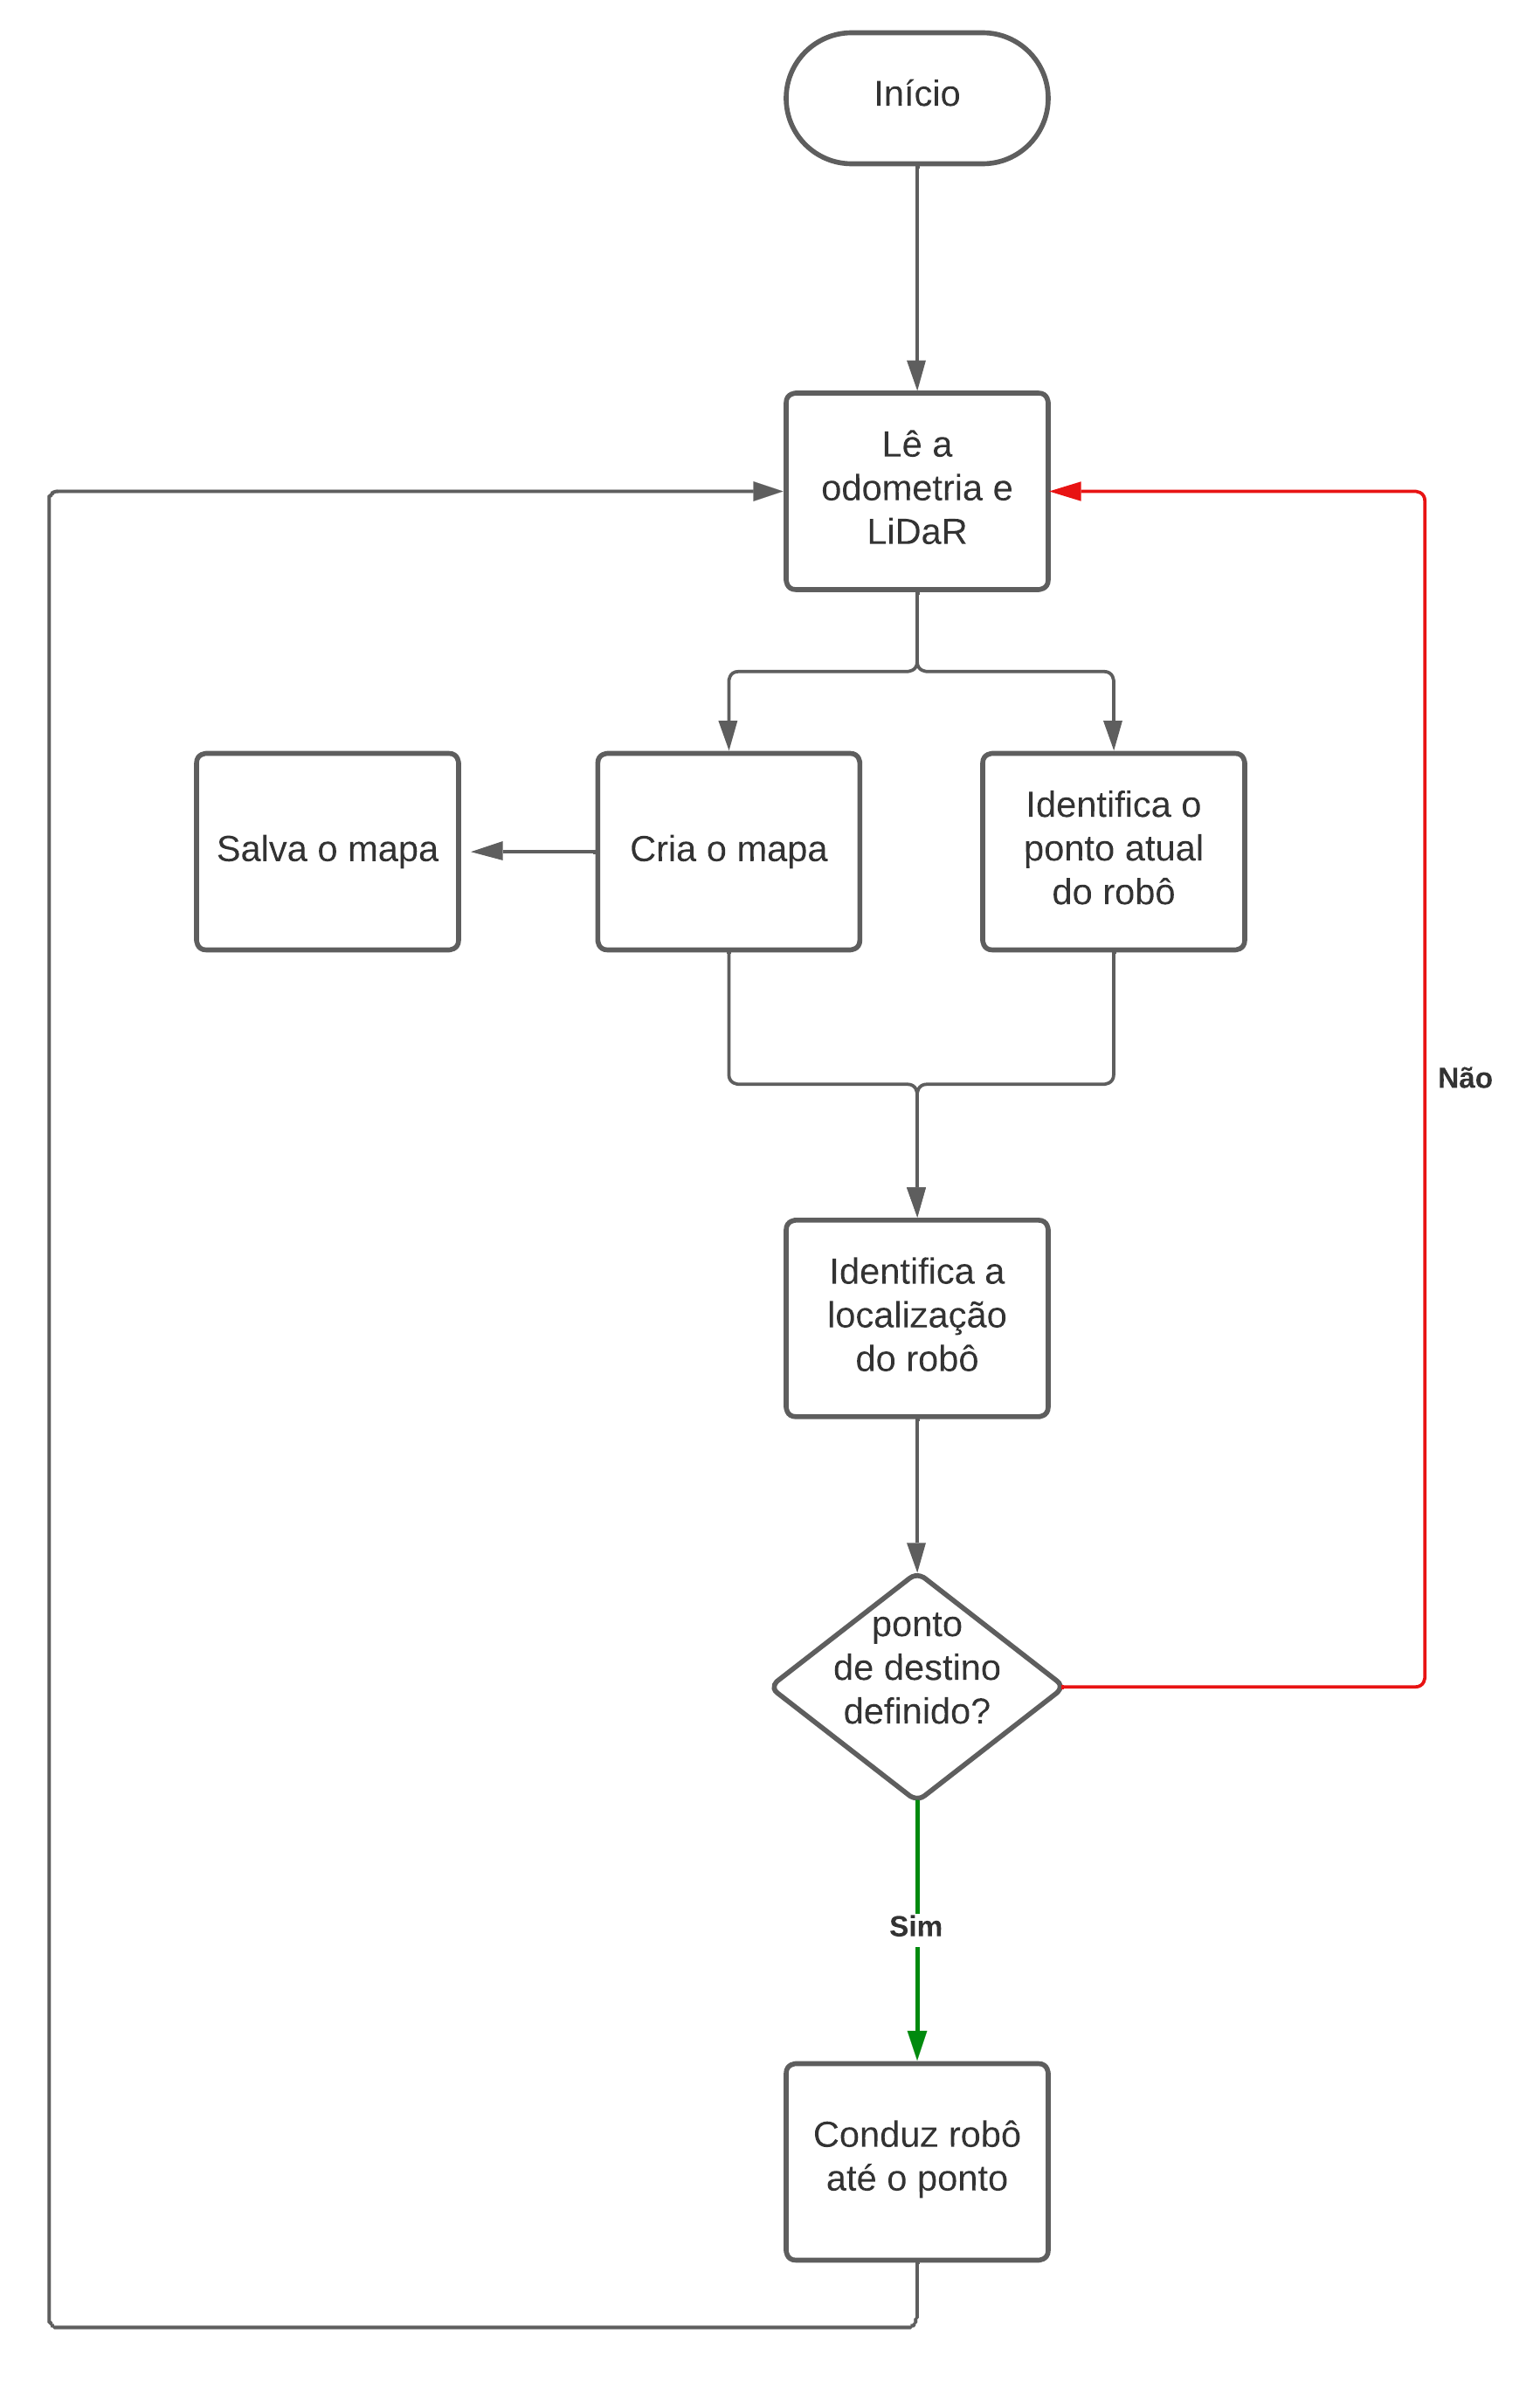
\includegraphics[scale=0.5]{fluxogramaComando.png}
   
    \caption*{Fonte: Autora (2023).}
    \label{fig:fluxogramaComando}
\end{figure}

\subsection{Sistema Operacional de Robô}

Visto a quantidade de singularidades, foi utilizado o ROS para integrar todos os componentes e conectá-los entre o robô e a simulação. Para isso, foram definidas as características do robô em termos que o ROS reconheça, por URDFs (formato de descrição de robô universal) traduzidos dos SDFs para a simulação. Essas descrições foram integradas com informações específicas dos sensores e odometria do robô, para serem acessadas pelas demais bibliotecas e o algoritmo de vagar.

O ROS é constituído por componentes (nomeados como nós) que se comunicam entre si por linhas de comunicação (tópicos) que podem ser acessadas para enviar novas informações (publicar) ou captar informações publicadas (inscrever) por outros nós. Para que essas comunicações entre os nós se tornem mais confiáveis e robustas, foram utilizadas as configurações de qualidade de serviço  a partir do \textit{middleware} Cyclone \cite{qos, cyclone}.

Por fim, a estrutura do modelo proposto é composta pelo robô e o ambiente configurados por arquivos que descrevem todas as suas características importantes. Através do ROS e seu \textit{middleware}, as informações do ambiente simulado são capturadas pelos sensores e são comunicados para as bibliotecas de SLAM e navegação, além do algoritmo de vagar sem colisão. Assim como, os comandos necessários para o robô se mover são repassados pelo intermédio do sistema operacional de robô.

Na Figura~\ref{fig:diagramaBlocosDetalhado}, é encontrada a integração entre todos os componentes supracitados. Em azul, estão as leituras realizadas pelo sensor LiDaR para percepção do ambiente e identificação de obstáculos. Também é representada a odometria, em rosa, coletada pelas informações das rodas. Ambos dados são utilizados pela biblioteca Slam Toolbox e o algoritmo de vagar sem colisões, pelo intermédio do ROS. Assim como, em verde, a velocidade nas rodas é inferida através da definição de seu valor pelo algoritmo de vagar sem colisão ou pela biblioteca Nav2.

\begin{figure}[h]
    \centering
    \caption{Diagrama da integração dos componentes do AtmosBot}
    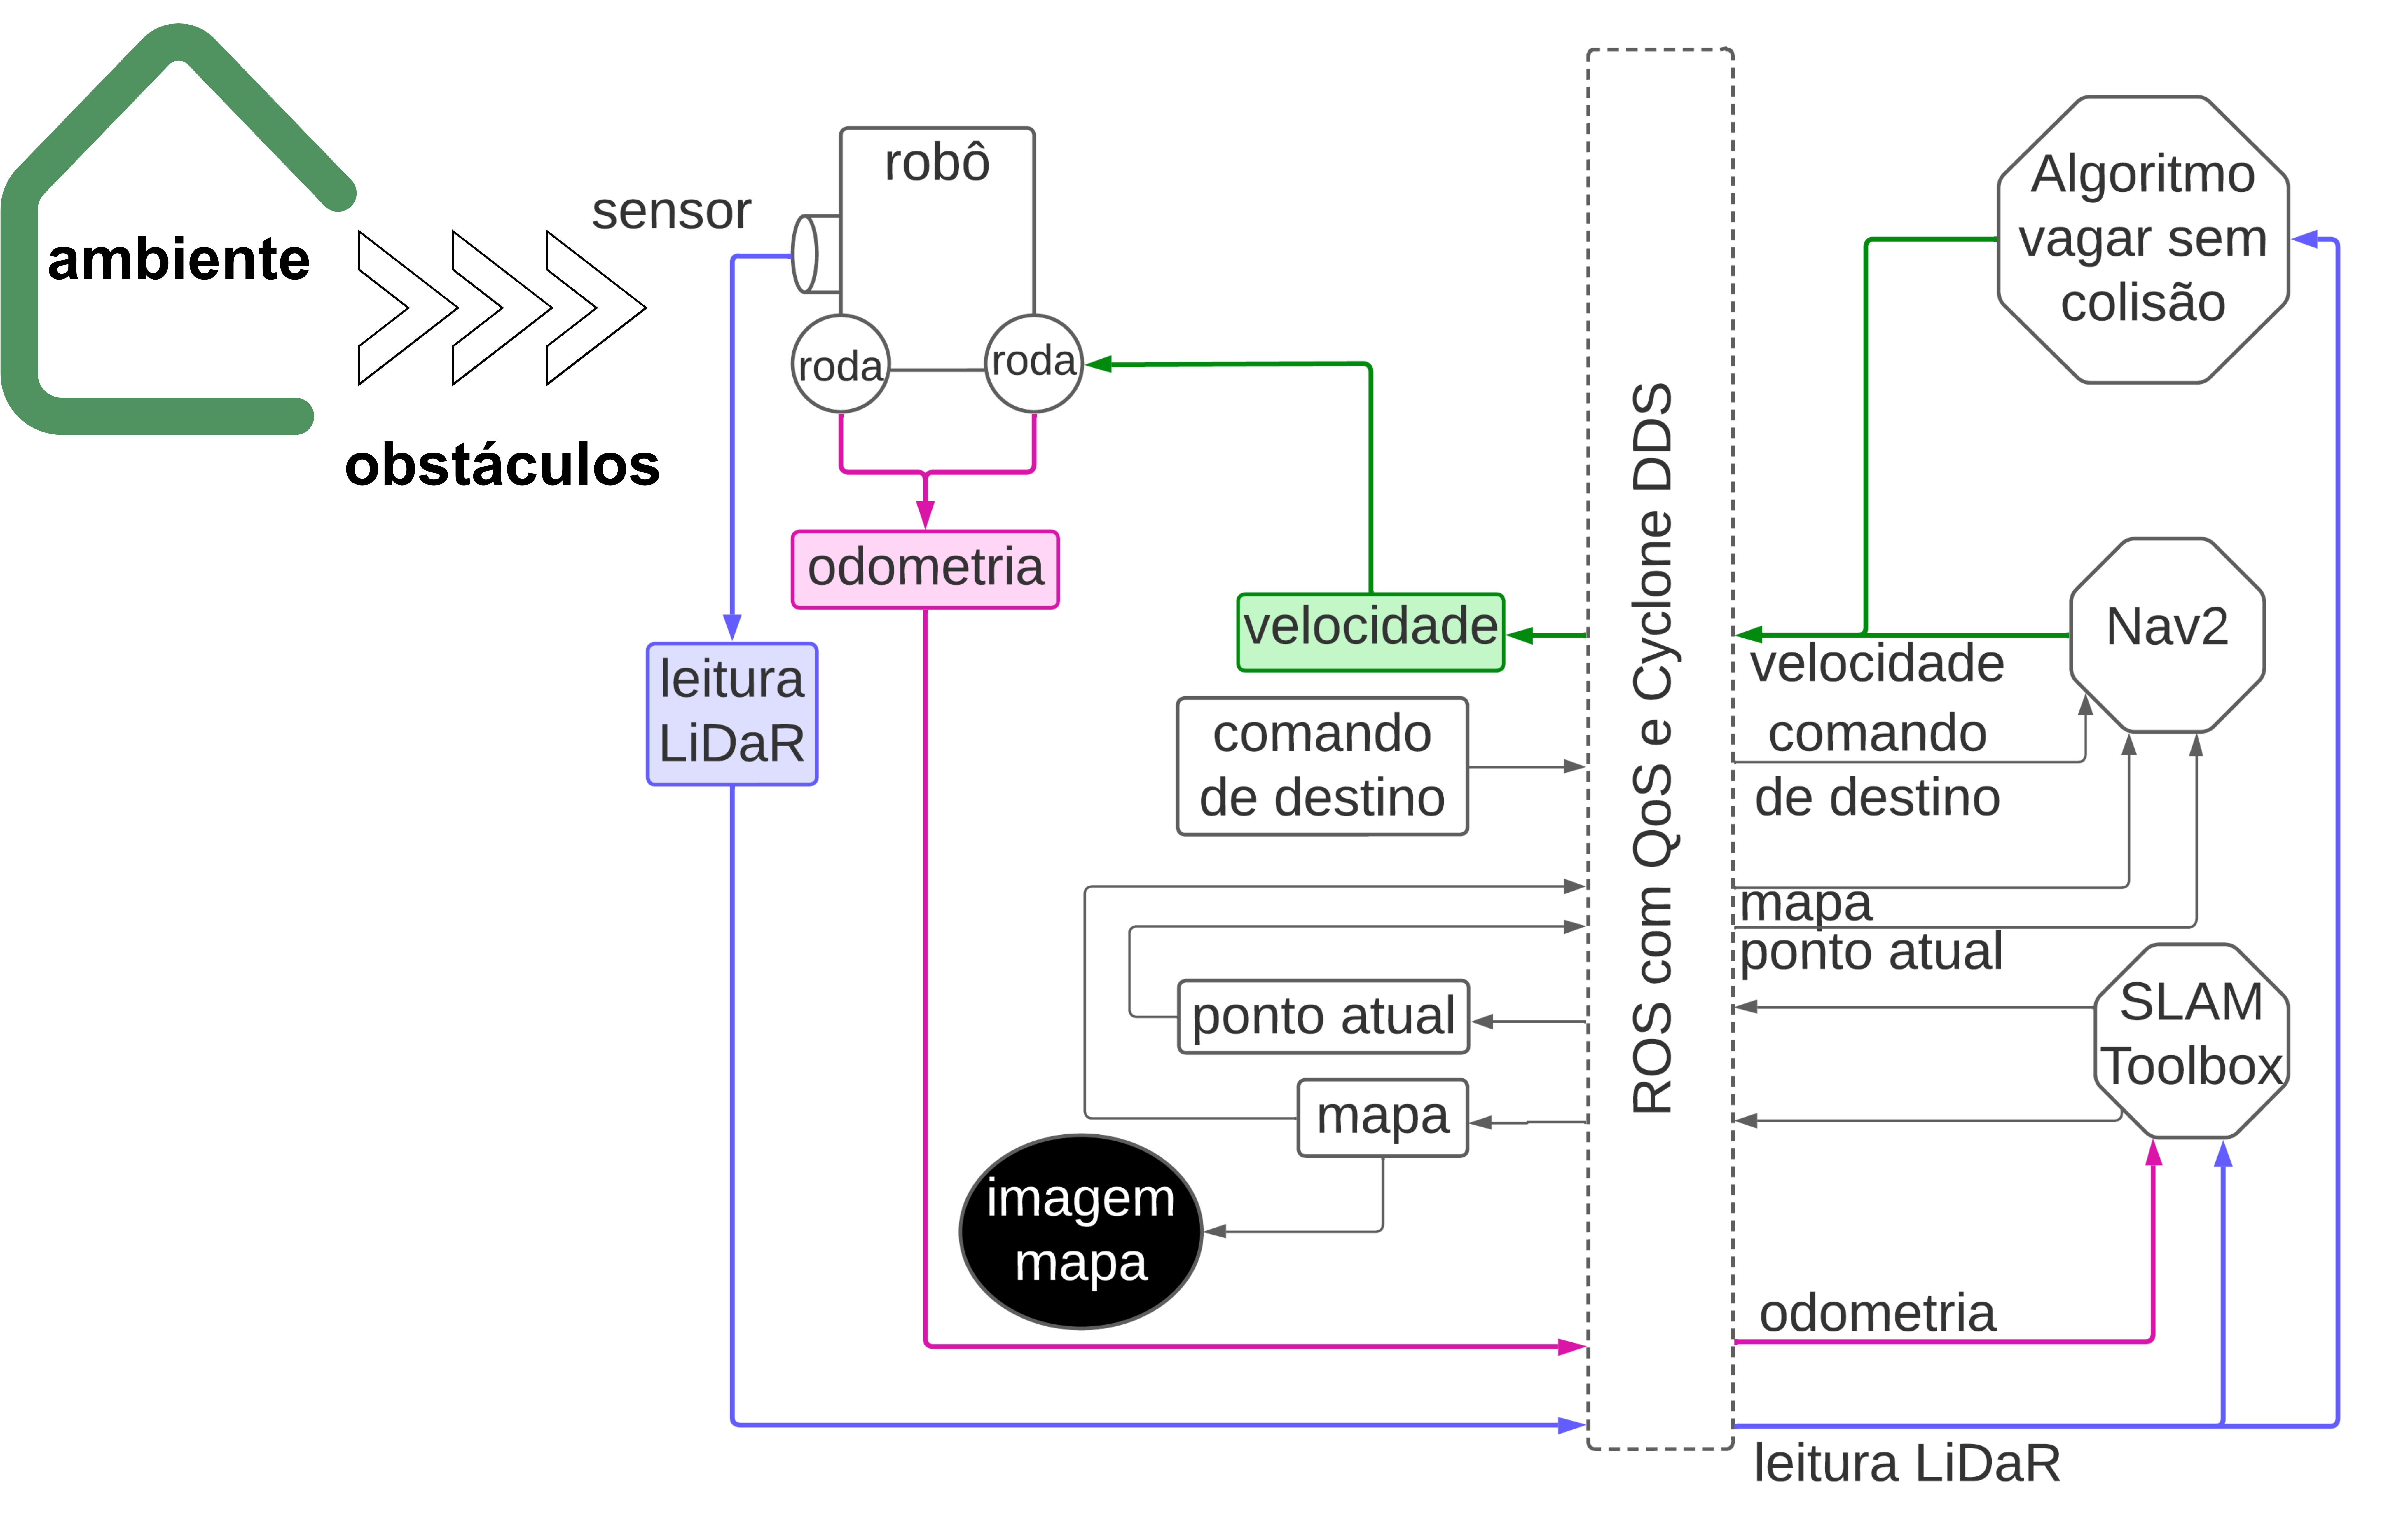
\includegraphics[scale=0.6]{diagramaBlocosDetalhado.png}
    
    \caption*{Fonte: Autora (2023).}
    \label{fig:diagramaBlocosDetalhado}
\end{figure}